\documentclass[12pt]{iopart}
\usepackage{graphicx}
\usepackage[margin=2.5cm]{geometry}
%\usepackage{natbib} %aas uses natbib
\usepackage{setstack}


% paragraph spacing
\setlength{\parskip}{.7em}
\setlength{\parindent}{0em}

% maths/symbols

\usepackage{amssymb}

% figures
\usepackage{graphicx}
\graphicspath{{./figures/}}
\usepackage{subcaption} % subfigures

% positioning of figures and tables
\usepackage{float}

% hyperlinks
\usepackage{hyperref}


\date{October 2023}




\begin{document}
\title{Mid-Infrared Analysis of Accreting Supermassive Black Holes}
\author{Mitchell Hooymans $^1$, Michael Cowley (Supervisor) $^1$}
\address{$^1$ Queensland University of Technology, Brisbane, Australia, 4000}

\begin{abstract}
    Abstract of this Project
\end{abstract}

\ioptwocol
\section{Introduction}
Accreting Supermassive Black Holes, also called Active Galactic Nuclei (AGN), are incredibly compact and energetic regions of space that exist in the centre of some galaxies. These supermassive objects are surrounded by diffuse material that spirals toward the centre, the transfer of angular momentum by the material causes it to heat up forming an ultra hot accretion disc \cite{shakura_black_1973}. Outside of this accretion disc lies a doughnut-like structure of gas and dust, known as the dusty torus. This dusty torus extends from a few parsecs to a hundred parsecs from the central area of the AGN \cite{netzer_revisiting_2015}. Dust from the dusty torus can obscure AGN preventing these objects from being observed. Fortunately, emissions from the galactic nuclei are absorbed by the surrounding dusty torus and re-emit in the mid-infrared which has a distinctive spectral energy \cite{lyu_polar_2018}. Due to the infrared colours that are produced by AGN in this way it is often possible to separate AGN observations from that of luminous star-forming galaxies \cite{hickox_obscured_2018}.
Due to this distinctive energy distribution we can observe these galaxies in specific infrared colour bands, and create criteria to select AGN candidates using the fluxes in these colour bands \cite{lacy_obscured_2004, stern_midinfrared_2005, donley_identifying_2012, messias_new_2012}. In addition to IR selection techniques, x-ray selection techniques are thought to be a robust method for selecting AGN with x-ray AGN signatures often being present in AGN identified with other wavelength techniques such as infrared, optical or radio \cite{brandt_cosmic_2015}. In this paper, we attempt to select AGN from the Fourstar Galaxy Evolution Survey (ZFOURGE) \cite{straatman_fourstar_2016} using IR and x-ray techniques. To facilitate the x-ray selections we cross-match data from the Chandra Deep Field South 4Ms Source Catalogue \cite{xue_chandra_2011} to determine x-ray data for sources present in ZFOURGE. 
\section{Data}
\subsection{ZFOURGE}
For this project, the data we used was from the ZFOURGE Survey \cite{straatman_fourstar_2016}. This survey observed over 60000 galaxies in three legacy fields, CDFS \cite{giacconi_chandra_2002}, COSMOS \cite{scoville_cosmic_2007}, and UDS \cite{lawrence_ukirt_2007} each pointing covering $11' \times 11'$. Observations in ZFOURGE were made using the FourStar Infrared Camera mounted on the Magellan Baade Telescope in Las Campanas, Chile \cite{persson_fourstar_2013}. Using the FourStar instrument, ZFOURGE observes with five near-infrared medium band filters; $J_1$, $J_2$, $J_3$, $H_s$, $H_l$ and one broad band filter $K_s$. In addition to this, the ZFOURGE survey is supplemented with multiwavelength data from CANDELS \cite{grogin_candels_2011, koekemoer_candels_2011} and data from the Spitzer Space Telescope's IRAC \cite{fazio_infrared_2004} and MIPS \cite{rieke_multiband_2004} instruments. Additional information regarding the ZFOURGE survey, including a complete list of auxiliary data and processing, can be found in Straatman's ZFOURGE paper \cite{straatman_fourstar_2016}.
\subsection{Crossmatching}
X-ray data was crossmatched from the Chandra Deep Field-South 4Ms Survey \cite{xue_chandra_2011} with ZFOURGE data in the CDFS field to allow the selection of AGN that produce x-ray emissions. To accomplish this both catalogues were imported and crossmatching was accomplished by matching celestial coordinates using the Astropy package \cite{the_astropy_collaboration_astropy_2013}. Performing this cross-match yielded an average sepeation between matches of around 0.4 arcseconds shown in Figure 1. 
\begin{figure}[h]
  \centering
  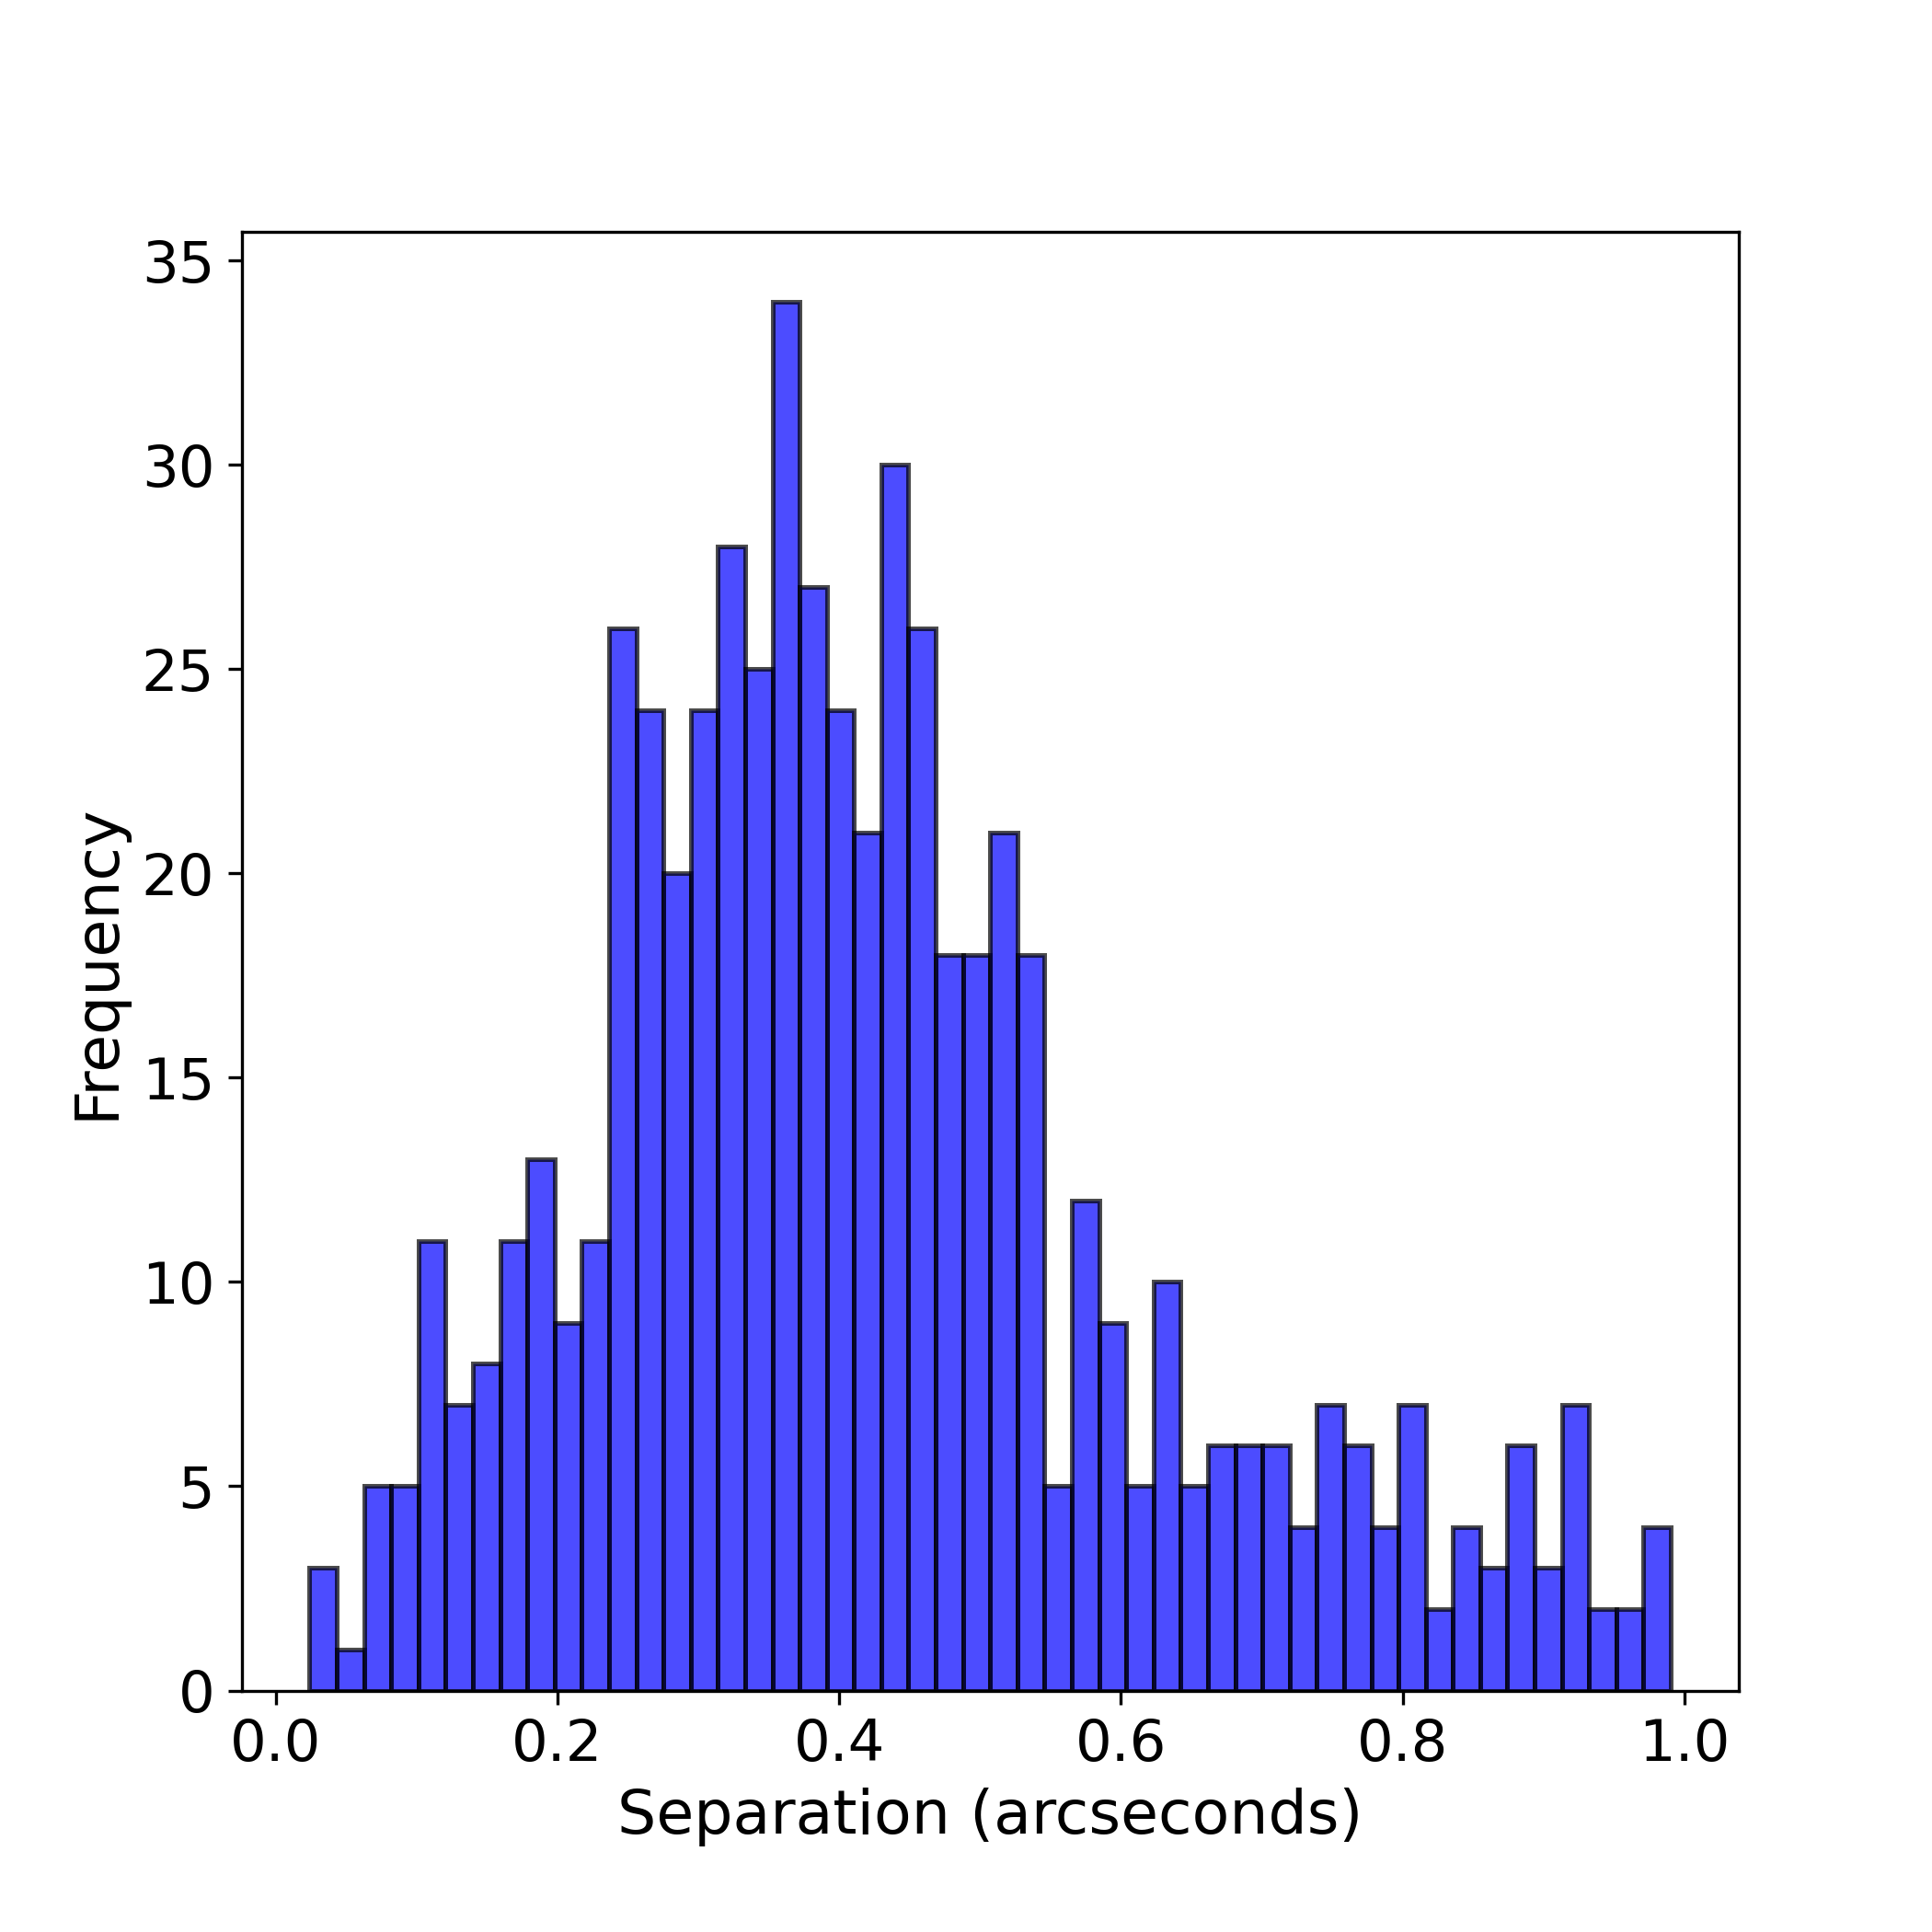
\includegraphics[width=0.53\textwidth]{plots/CDFS_4Ms_Xray_Sep.png}
  \caption{Your figure caption here.}
  \label{fig:your_label}
\end{figure}


\newpage
\section{Selection of AGN Candidates}
\subsection{Infrared Selection}
\subsection{X-Ray Selection}
\section{Results}
\section{Discussion}
\section{Conclusion}
\section{Acknowledgements}
\section{References}
\bibliographystyle{vancouver}
\bibliography{report/references}
%\bibliography{references.bib} % references file!

%\bibliographystyle{vancouver} % referencing style


\end{document}